\documentclass[
  captions=tableheading,
  bibliography=totoc, 
  titepage=firstiscover,
]{scrartcl}

\usepackage{blindtext} %neuer input

\usepackage{longtable} % Tabellen über mehrere Seiten

\usepackage[utf8]{inputenc} %neuer input

\usepackage{scrhack}

\usepackage[aux]{rerunfilecheck} %Warnung falls nochmal kompiliert werden muss

\usepackage{fontspec} %Fonteinstellungen

\recalctypearea{}

\usepackage[main=ngerman]{babel} %deutsche Spracheinstellung

\usepackage{ragged2e} %neuer input

\usepackage{amsmath, nccmath}

\usepackage{amssymb} %viele mathe Symbole

\usepackage{mathtools} %Erweiterungen für amsmath


\DeclarePairedDelimiter{\abs}{\lvert}{\rvert}
\DeclarePairedDelimiter{\norm}{\lVert}{\rVert}

\DeclarePairedDelimiter{\bra}{\langle}{\rvert}
\DeclarePairedDelimiter{\ket}{\lvert}{\rangle}

\DeclarePairedDelimiterX{\braket}[2]{\langle}{\rangle}{
#1 \delimsize| #2
}

\NewDocumentCommand \dif {m}
{
\mathinner{\symup{d} #1}
}


\usepackage[
  math-style=ISO,
  bold-style=ISO,
  sans-style=italic,
  nabla=upright,
  partial=upright,
  warnings-off={
    mathtools-colon,
    mathtools-overbracket,
  },
]{unicode-math}

\setmathfont{Latin Modern Math}
\setmathfont{XITS Math}[range={scr, bfscr}]
\setmathfont{XITS Math}[range={cal, bfcal}, StylisticSet=1]


\usepackage[
  locale=DE,
  separate-uncertainty=true,
  per-mode=reciprocal,
  output-decimal-marker={,},
]{siunitx}

\usepackage[autostyle]{csquotes} %richtige Anführungszeichen

\usepackage{xfrac}

\usepackage{float}

\floatplacement{figure}{htbp}

\floatplacement{table}{htbp}

\usepackage[ %floats innerhalb einer section halten
  section,   %floats innerhalb er section halten
  below,     %unterhalb der Section aber auf der selben Seite ist ok
]{placeins}

\usepackage[
  labelfont=bf,
  font=small,
  width=0.9\textwidth,
]{caption}

\usepackage{subcaption} %subfigure, subtable, subref

\usepackage{graphicx}

\usepackage{grffile}

\usepackage{booktabs}

\usepackage{microtype} %Verbesserungen am Schriftbild

\usepackage[
backend=biber,
]{biblatex}

\addbibresource{../lit.bib}

\usepackage[ %Hyperlinks im Dokument
  german,
  unicode,
  pdfusetitle,
  pdfcreator={},
  pdfproducer={},
]{hyperref}

\usepackage{bookmark}

\usepackage[shortcuts]{extdash}

%\usepackage{warpcol}


\begin{document}
    \title{ATP Übungsblatt 4}
    \author{  
    Tobias Rücker\\
    \texorpdfstring{\href{mailto:tobias.ruecker@tu-dortmund.de}{tobias.ruecker@tu-dortmund.de}
    \and}{,} 
    Paul Störbrock\\
    \texorpdfstring{\href{mailto:paul.stoerbrock@tu-dortmund.de}{paul.stoerbrock@tu-dortmund.de}}{}
    }
\maketitle
\center{\Large Abgabegruppe: \textbf{Mittw. 10-12 Uhr}}
\thispagestyle{empty}

\newpage
\tableofcontents
\thispagestyle{empty}
\newpage

\setcounter{page}{1}

\section{Aufgabe 13}

    \begin{figure}[H]
        \centering
        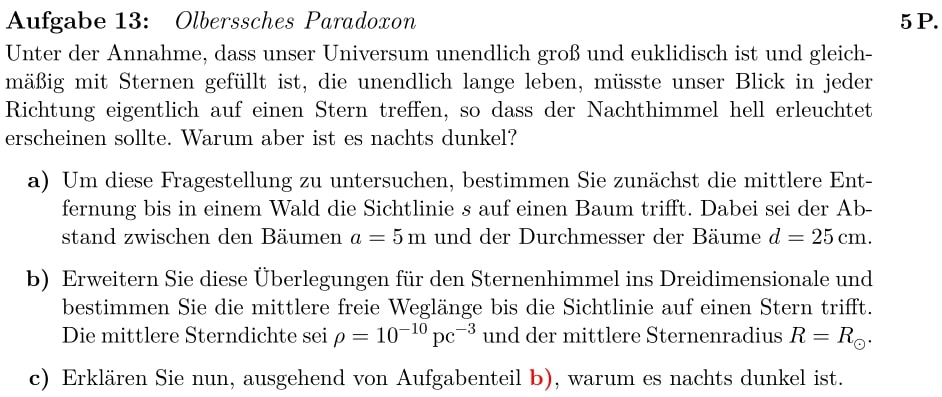
\includegraphics[width=\textwidth]{images/Aufgabe13.jpg}
        \label{fig:1}
    \end{figure}

\subsection{a)}

    \flushleft{Bei\;}\justifying der Wald-Analogie des Olbersschen Paradoxon wird die Formel der mittleren freien Weglänge im 2-Dimensionalen
    verwendet:
    \begin{align*}
        \lambda &= \frac{1}{\rho\cdot\sigma}
    \end{align*}
    \flushleft{Hierbei\;}\justifying ist $\rho$ die Baumdichte des Waldes und $\sigma$ der Wirkungsquerschnitt eines Baumes (\SI{25}{\centi\meter}).
    Um die Baumdichte bestimmen zu können, wird eine Fläche vorrausgesetzt. Hier wird eine Approximation der Fläche des Stadtwaldes von Dattel
    verwendet. Die Fläche des Lohbusches ist ungefähr:
    \begin{align*}
    \text{Länge} &= \text{\input{Länge.tex}}\\
    \text{Breite} &= \text{\input{Breite.tex}}\\
    \text{Fläche} &= \text{\input{Fläche.tex}}
    \intertext{
        \flushleft{Aus\;}\justifying der Fläche lässt sich über die Teilchenzahl $N$ die Baumdichte mithilfe von
    }
    \rho &= \frac{N}{A}
    \intertext{
        \flushleft{bestimmen.\;}\justifying Da die Baumverteilung als homogen bei einem Abstand von \SI{5}{\meter} angenommen wird,
        ist die Baumzahl $N$ hiermit:
    }
    N &= \frac{A}{25} = \text{\input{Baumzahl.tex}}
    \intertext{
        \flushleft{Die\;}\justifying Baumdichte ist damit:
    }
    \rho &= \text{\input{Baumdichte.tex}}\\
    \Rightarrow \lambda &= \frac{1}{\rho\cdot\sigma} = \text{\input{lambda.tex}}
    \end{align*}


\subsection{b)}

    \flushleft{Wird\;}\justifying das Analogon aus Aufgabenteil a) auf den 3-dimensionalen Raum des Universums angewandt, bei einer 
    mittleren Sternendichte von $\rho = 10^{-10}\text{pc}^{-3}$ und einem mittleren Sternenradius $R=R_{\odot}$, ergibt
    sich für die mittlere Entfernung:
    \begin{align*}
        \lambda &= \frac{1}{\rho \sigma}\\
        \sigma &= \pi\cdot R_{\odot}^2 = \text{\input{sigma_13b.tex}}\\
        \Rightarrow\lambda &= \text{\input{lambda_13b.tex}}
        \intertext{
            \flushleft{In\;}\justifying Parsec ergibt das:
        }
        \Rightarrow\lambda &= \text{\input{lambda_13b_parsec.tex}}
    \end{align*}

\subsection{c)}

    \flushleft{Der\;}\justifying Grund, dass der Nachhimmel dunkel ist, liegt an der falschen Annahme des Paradoxons, dass das Universum 
    unendlich alt ist. Mit einem geschätzten Alter von 15 milliarden Jahren, hat das momentane Universum einen Radius von ca. 15 milliarden
    Lichtjahren. Wird nun die mittlere freie Weglänge aus b) in Lichtjahre umgerechnet, ergibt sich:
    \begin{align*}
        \lambda &= \text{\input{lambda_13c.tex}}\\
        \frac{15\cdot 10^9\text{ly}}{\text{\input{lambda_13c}}\cdot 100} &= \text{\input{percent.tex}}
    \end{align*}
    \flushleft{Aus\;}\justifying dem Prozentsatz vom Alter des Universums über der mittleren freien Weglänge lässt sich schließen,
    dass das Licht der Sterne außerhalb des observablen Universums, im Falle eines unendlichen Universums, nicht die Zeit hatte,
    uns zu erreichen. 


\section{Aufgabe 14}

    \begin{figure}[H]
        \centering
        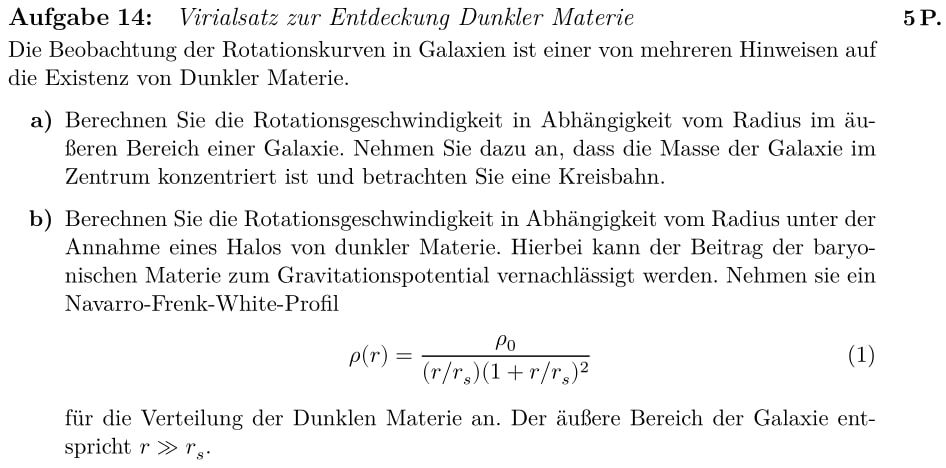
\includegraphics[width=\textwidth]{images/Aufgabe14ab.jpg}
        \label{fig:2}
    \end{figure}

    \begin{figure}[H]
        \centering
        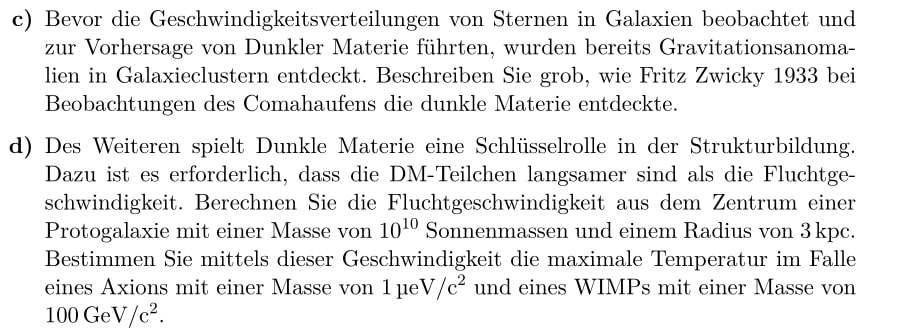
\includegraphics[width=\textwidth]{images/Aufgabe14cd.jpg}
        \label{fig:3}
    \end{figure}

\subsection{a)}


\subsection{b)}

\subsection{c)}

\subsection{d)}

\section{Aufgabe 15}

    \begin{figure}[H]
        \centering
        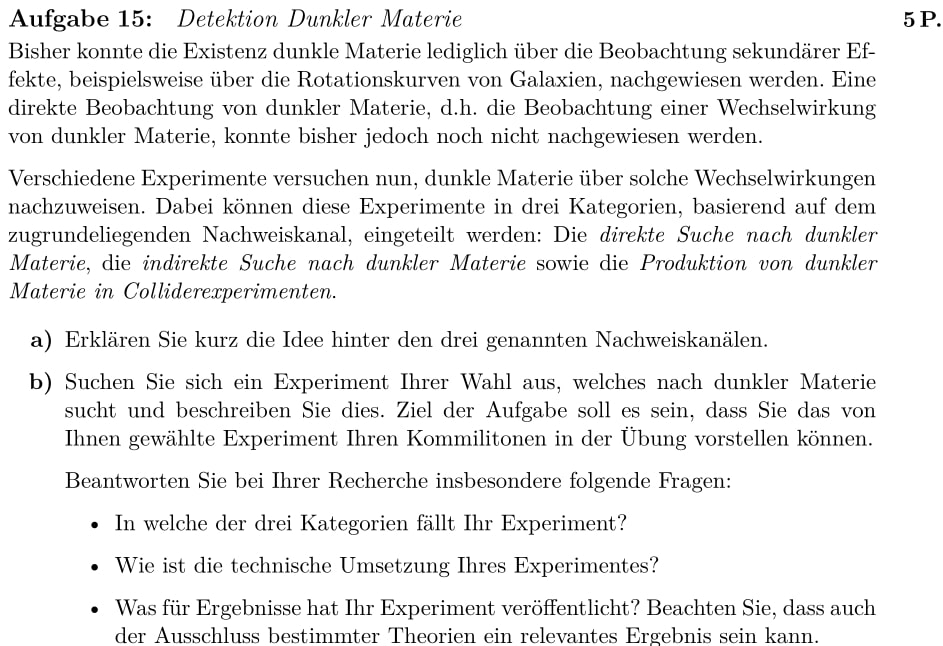
\includegraphics[width=\textwidth]{images/Aufgabe15.jpg}
        \label{fig:4}
    \end{figure}

\subsection{a)}

\subsection{b)}

\end{document}